\documentclass{article}[18pt]
\ProvidesPackage{format}
%Page setup
\usepackage[utf8]{inputenc}
\usepackage[margin=0.7in]{geometry}
\usepackage{parselines} 
\usepackage[english]{babel}
\usepackage{fancyhdr}
\usepackage{titlesec}
\hyphenpenalty=10000

\pagestyle{fancy}
\fancyhf{}
\rhead{Sam Robbins}
\rfoot{Page \thepage}

%Characters
\usepackage{amsmath}
\usepackage{amssymb}
\usepackage{gensymb}
\newcommand{\R}{\mathbb{R}}

%Diagrams
\usepackage{pgfplots}
\usepackage{graphicx}
\usepackage{tabularx}
\usepackage{relsize}
\pgfplotsset{width=10cm,compat=1.9}
\usepackage{float}

%Length Setting
\titlespacing\section{0pt}{14pt plus 4pt minus 2pt}{0pt plus 2pt minus 2pt}
\newlength\tindent
\setlength{\tindent}{\parindent}
\setlength{\parindent}{0pt}
\renewcommand{\indent}{\hspace*{\tindent}}

%Programming Font
\usepackage{courier}
\usepackage{listings}
\usepackage{pxfonts}

%Lists
\usepackage{enumerate}
\usepackage{enumitem}

% Networks Macro
\usepackage{tikz}


% Commands for files converted using pandoc
\providecommand{\tightlist}{%
	\setlength{\itemsep}{0pt}\setlength{\parskip}{0pt}}
\usepackage{hyperref}

% Get nice commands for floor and ceil
\usepackage{mathtools}
\DeclarePairedDelimiter{\ceil}{\lceil}{\rceil}
\DeclarePairedDelimiter{\floor}{\lfloor}{\rfloor}

% Allow itemize to go up to 20 levels deep (just change the number if you need more you madman)
\usepackage{enumitem}
\setlistdepth{20}
\renewlist{itemize}{itemize}{20}

% initially, use dots for all levels
\setlist[itemize]{label=$\cdot$}

% customize the first 3 levels
\setlist[itemize,1]{label=\textbullet}
\setlist[itemize,2]{label=--}
\setlist[itemize,3]{label=*}

% Definition and Important Stuff
% Important stuff
\usepackage[framemethod=TikZ]{mdframed}

\newcounter{theo}[section]\setcounter{theo}{0}
\renewcommand{\thetheo}{\arabic{section}.\arabic{theo}}
\newenvironment{important}[1][]{%
	\refstepcounter{theo}%
	\ifstrempty{#1}%
	{\mdfsetup{%
			frametitle={%
				\tikz[baseline=(current bounding box.east),outer sep=0pt]
				\node[anchor=east,rectangle,fill=red!50]
				{\strut Important};}}
	}%
	{\mdfsetup{%
			frametitle={%
				\tikz[baseline=(current bounding box.east),outer sep=0pt]
				\node[anchor=east,rectangle,fill=red!50]
				{\strut Important:~#1};}}%
	}%
	\mdfsetup{innertopmargin=10pt,linecolor=red!50,%
		linewidth=2pt,topline=true,%
		frametitleaboveskip=\dimexpr-\ht\strutbox\relax
	}
	\begin{mdframed}[]\relax%
		\centering
		}{\end{mdframed}}



\newcounter{lem}[section]\setcounter{lem}{0}
\renewcommand{\thelem}{\arabic{section}.\arabic{lem}}
\newenvironment{defin}[1][]{%
	\refstepcounter{lem}%
	\ifstrempty{#1}%
	{\mdfsetup{%
			frametitle={%
				\tikz[baseline=(current bounding box.east),outer sep=0pt]
				\node[anchor=east,rectangle,fill=blue!20]
				{\strut Definition};}}
	}%
	{\mdfsetup{%
			frametitle={%
				\tikz[baseline=(current bounding box.east),outer sep=0pt]
				\node[anchor=east,rectangle,fill=blue!20]
				{\strut Definition:~#1};}}%
	}%
	\mdfsetup{innertopmargin=10pt,linecolor=blue!20,%
		linewidth=2pt,topline=true,%
		frametitleaboveskip=\dimexpr-\ht\strutbox\relax
	}
	\begin{mdframed}[]\relax%
		\centering
		}{\end{mdframed}}
\lhead{Networks and Systems - Distributed Systems}
\newcolumntype{b}{X}
\newcolumntype{s}{>{\hsize=.5\linewidth}X}

\begin{document}
\begin{center}
\underline{\huge Load Distribution}
\end{center}
\begin{definition}[Load Distribution]
Transfer load (tasks) from heavily loaded servers to idle or lightly loaded ones
\end{definition}
\begin{definition}[Load sharing]
Reduce the likelihood of an unshared state (e.g. idle servers)
\end{definition}
\begin{definition}[Load balancing]
Go a step further than load sharing by attempting to equalise loads at all servers
\end{definition}
\section{Where does the workload come from}
\begin{enumerate}
	\item Queue length of waiting tasks: proportional to response time
	\item CPU Utilisation
	\item Network bandwidth utilisation
\end{enumerate}
Load information collection:
\begin{itemize}
	\item \textbf{Central coordinator}: collects server load information centrally and globally
	\item \textbf{Local approach}: a server locally collects load information of neighbouring servers
\end{itemize}
\section{Simple task transfer}
\begin{definition}[Non-preemptive task transfers]
Transfer tasks that have not started executing
\begin{itemize}
	\item Transfer only the request(or task) without processing states
	\item Good for load sharing but difficult for load balancing
\end{itemize}
\end{definition}
\begin{definition}[Preemptive task transfers]
Transfer tasks that are partially executed - this is expensive as it involves collection and transmission of task states
\end{definition}
\begin{center}
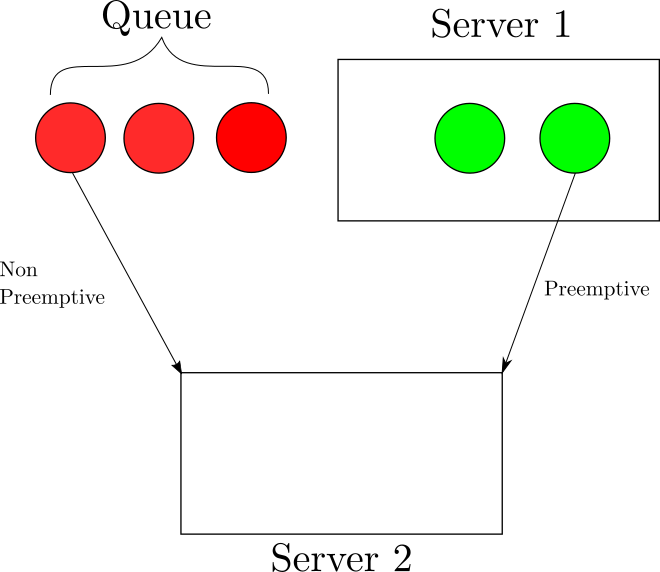
\includegraphics[scale=0.4]{preemptive}
\end{center}
\section{Routing mechanisms based on network network packet content}
Layer-4 routing
\begin{itemize}
	\item Determines the target server without referring the message/request content
	\item \textbf{Content-blind routing}: server selection is purely based on information from the IP header
\end{itemize}
Layer 7 Routing:
\begin{itemize}
	\item Examine a request at the application level and select a server accordingly
	\item Can support sophisticated dispatching policies, but may induce significant latency (also called content aware routing)
\end{itemize}
\subsection{Implementations}
\begin{definition}[Two-way]
Response from FE
\end{definition}
\begin{definition}[One-way]
Response from the server directly
\end{definition}
Two way is less scalable because of the overhead in the front end\\
\\
Layer 4 vs Layer 7 routing:
\begin{itemize}
	\item Layer 4 routing is efficient and requires only simple FE servers
	\item Layer 7 routing is less scalable
	\item Layer 7 routing benefits from server specialisation and content partition
\end{itemize}
\begin{tabularx}{\textwidth}{|X|X|X|X|X|X|}
	\hline
	Layer & Approach & Routing & Data Flow & Pros & Cons \\
	\hline
	Layer 4 & Two way & Content blind & inbound/ outbound & flexible, portable & switching throughout, TCP connection grain control \\
	\hline
	Layer 4 & One way & Content blind & inbound & simple, fast routing & network topology, TCP connection grain control \\
	\hline
	Layer 7 & Two way & Content aware & inbound/ outbound & simple, caching, server specialisation, content partition, SSL session reuse & switching bottleneck, slowest routing \\
	\hline
	Layer 7 & One way & Content aware & inbound & server specialisation, content partition, SSL session reuse & Switching bottleneck, complex routing \\
	\hline
\end{tabularx}
\section{Approaches for load distribution}
Static:
\begin{itemize}
	\item Decisions are hard-coded into an algorithm
	\item Simple in implementation
	\item A prior knowledge of system is required
\end{itemize}
Dynamic:
\begin{itemize}
	\item Make decision during runtime based on system states
	\item Correctness of load distribution depends on the timeliness of parameters collected
\end{itemize}
Adaptive:
\begin{itemize}
	\item Enhance the dynamic approach by allowing making choices of decision algorithms and the frequency of collecting load information based on system states
\end{itemize}
\section{Constructing a load distribution algorithm}
Four main components:
\begin{itemize}
	\item Transfer
	\item Selection
	\item Location
	\item Information policies
\end{itemize}
These define what information is required to collect and maintain supporting decision making, and what procedures are required to follow for distributing workload
\subsection{Transfer policy}
Decide whether a server needs to transfer tasks
\begin{itemize}
	\item Thresholds: number of tasks, processor utilisation
	\item Role: a server becomes sender/receiver when its load over/under a threshold
	\item Issue: sensitive to time duration of a task transfer
\end{itemize}
\subsection{Selection policy}
Determines which task(s) to transfer
\begin{itemize}
	\item Tasks cause a server overload
	\item Estimated task execution time
	\item Or serve response time improvement
	\item Minimise location-dependent system calls made by the selected task
\end{itemize}
\subsection{Location policy}
Decide the receiving server for a task
\begin{itemize}
	\item Polling is generally used
	\item Can be done serially or in parallel(using multicast)
\end{itemize}
\subsection{Information policy}
Decide when, where and what information to collect
\begin{itemize}
	\item Demand-driven: a server collects the state of other servers only when it becomes either a se4nder or receiver
	\item Periodic: servers exchange load information periodically
	\item State-change-driven: servers disseminate state information whenever their state changes by a certain degree
\end{itemize}
\section{Load distributing algorithms}
\begin{definition}[Sender-initiated]
	Distribution initiated by an overloaded server
\end{definition}
\begin{definition}[Receiver-initiated]
	Distribution initiated by lightly loaded servers
\end{definition}
\begin{definition}[Symmetric]
	Initiated by both senders and receivers. Has advantages and disadvantages of both the approaches
\end{definition}
\begin{definition}[Adaptive]
	Sensitive to the state of the system
\end{definition}
\subsection{Sender and Receiver Initiated}
{\renewcommand{\arraystretch}{2}
\begin{tabular}[t]{ | m{5em} | m{22em}| m{22em} | } 
\hline
&Sender Initiated&Receiver Initiated\\
\hline
Transfer Policy& Use thresholds
\begin{itemize}
	\item \textbf{Sender} if queue length exceeds threshold T
	\item \textbf{Receiver} if accepting a task will not make queue length exceed T 
\end{itemize}
& Use thresholds
\begin{itemize}
	\item \textbf{Receiver} if queue length below T
	\item \textbf{Sender} if queue length above T
\end{itemize}
\\
\hline
Selection policy& Only newly arrived tasks& Only newly arrived tasks\\
\hline
Location policy&
Identify receiver
\begin{itemize}
	\item Random: Task transferred to server at random
	\begin{itemize}
		\item No need for state collection
		\item Unnecessary task transfers may occur
	\end{itemize}
	\item Threshold: Poll a server to find out if it is a receiver, Receiver must accept the task irrespective of when the task actually arrives
	\item Shortest: Poll servers. Select the receiver with shortest task queue length
\end{itemize}
&
Polling:
\begin{itemize}
	\item Poll a random server, transferring a task transfer when queue length $>$ threshold
	\item Repeat the process to attempt transferring tasks from another server until PollLimit is reached
\end{itemize}\\
\hline
Information Policy& demand-driven&demand-driven\\


\hline
Stability& Can become unstable at high loads
\begin{itemize}
	\item At high loads, it may become difficult for senders to find receivers
	\item Also, the number of senders increase at high system loads thereby increasing the polling activity
	\item Polling activity may make the system unstable at high loads
\end{itemize}&
"Not unstable" since there are lightly loaded systems that have initiated the algorithm\\
\hline
\end{tabular}
}
\subsection{Symmetric}
\begin{itemize}
	\item Senders search for receivers and vice-versa
	\item Low loads: senders can find receivers easily\\
	High loads: receivers can find senders easily
	\item May have the disadvantages of both
	\begin{itemize}
		\item Polling at high loads can make the system unstable
		\item Receiver-initiated task transfers can be preemptive and so expensive
	\end{itemize}
\end{itemize}
\subsection{Adaptive algorithm}
\textbf{Main idea}
\begin{itemize}
	\item Aim: Limit sender's polling actions at high load to avoid instability
	\item Classify servers based on the collected state information and poll adaptively
\end{itemize}
\textbf{The process}
\begin{itemize}
	\item Each server maintains three lists. All servers are assumed to be receivers initially
	\item Location policy at sender:
	\begin{itemize}
		\item Sender polls the head of the receiver list
		\item Polled server puts the sender at the head of its sender list, and informs the sender whether it is a receiver, a sender, or an OK server
		\item If the polled server is still a receiver, the new task is transferred
		\item Else sender updates lists and polls the next potential receiver
		\item If this polling process fails to identify a receiver, the task can still be transferred during a receiver-initiated dialogue
	\end{itemize}
	\item Location policy at receiver:
	\begin{itemize}
		\item Receivers obtain tasks from potential senders. Lists are scanned in the following order
		\begin{itemize}
			\item Head to tail in senders list (most up to date info used), tail to head in OK list (lead up to date used), tail to head in receiver list
			\item Least up to date used in the hope that status might have changed
		\end{itemize}
		\item Transfer a task if a sender is found
		\item If the server is not a sender, both the polled server and receiver update each other's status
		\item Polling process stops if a sender is found or a static PollLimit is reached
	\end{itemize}
\end{itemize}
At high loads, sender initiated polling gradually reduces as servers get removed from receiver list(and become senders) whereas at low loads, sender will generally find some receiver\\
\\
At high loads, receiver initiated works and can find a sender whereas at low loads receiver may not find senders, but that does not affect the performance\\
\\
Algorithm dynamically becomes sender-initiated at low loads and receiver-initiated at high loads\\
\\
Hence, algorithm is stable and can use non-preemptive transfers at low loads (sender initiated)
\section{Selecting an algorithm}
\begin{itemize}
	\item If a system never gets highly loaded, sender initiated algorithms work better
	\item Receiver-initiated algorithms are better for high loads
	\item Widely fluctuating loads: symmetric algorithms
	\item Widely fluctuating loads and high migration cost for preemptive transfers: sender-initiated algorithms
	\item Heterogeneous work arrival: adaptive algorithms
\end{itemize}
\end{document}